\chapter{Fundamentação Teórica} \label{cap:cap2}

Este Capítulo relaciona os conceitos e as tecnologias envolvidas no desenvolvimento do ambiente de treinamento proposto. 

\section{Anestesias Regionais}

Anestesias são atualmente usadas em diversos procedimentos cirúrgicos na medicina tradicional com o intuito de bloquear temporariamente a capacidade do cérebro de reconhecer um estímulo doloroso. Esta prática visa permitir a execução de procedimentos invasivos por parte do médico enquanto mantém o conforto e a tranquilidade do paciente. A anestesia regional é um procedimento usado em cirurgias onde o paciente pode permanecer acordado. Este tipo de anestesia bloqueia a dor em apenas uma determinada região do corpo, como um braço, uma perna ou toda região inferior do corpo, abaixo do abdômen \cite{Pinheiro2018}.

Os dois tipos de anestesias regionais mais usados são: anestesia raquidiana (ou raquianestesia, raqui), e anestesia peridural ou epidural. Estes dois tipos de anestesias também são conhecidas como anestesias de neuroeixo ou ainda bloqueio de neuroeixo \cite{Pinheiro2018}. Ambas podem ser aplicadas com pacientes sentados e inclinados para frente ou deitados de lado \cite{Anesclin2019}. 

Após a finalização dos procedimentos de preparação é escolhida a área onde será feita a punção através do toque da mão do médico na crista ilíaca do paciente \cite{Helayel2010,Isaacs2015}. Uma vez escolhido este ponto é feita a injeção de anestésico local para reduzir o desconforto na área próxima à punção (\cite{Sedicias2018} Após a anestesia local é feita a inserção da agulha de punção tanto no caso da peridural como na raqui.
Existem duas principais abordagens de inserção da agulha para efetuação das anestesias regionais. Estão são denominadas mediana (do inglês \textit{midline}) e paramediana (do inglês \textit{paramedian}). A abordagem mediana é utilizada com mais frequência (96\%) \cite{Wantman2006}. Um dos motivos para o maior uso da abordagem mediana é a ausência de vasos sanguíneos no caminho da agulha nesta abordagem \cite{Bapat2015}. A abordagem paramediana é mais recomendada para pacientes idosos \cite{Ahsan-ul-Haq2005} por motivos de modificação degenerativa da coluna vertebral \cite{Boon2003} e calcificação dos ligamentos interespinhoso e supraespinhoso \cite{Wantman2006}. A abordagem paramediana também pode ser mais viável que a mediana em pacientes obesos pela dificuldade na identificação da crista ilíaca nestes pacientes. Isto por que a camada de gordura faz com que a linha média seja mais difícil de localizar através do toque do médico \cite{N.2013}. Na abordagem mediana a agulha é inserida na linha média da coluna vertebral. Na paramediana existe certa angulação entre a linha da coluna e a inserção da agulha. As duas abordagens podem ser observadas no corte transversal da coluna na Figura 2 \cite{MedBroadcast2018}. 

===== FIGURA ====

\subsection{Anestesia Raquidiana}

Neste tipo de anestesia, uma agulha de pequeno calibre é inserida nas costas do paciente até atingir o espaço subaracnóideo (localizado após a dura-máter), dentro da coluna espinhal. Em seguida, um anestésico é injetado dentro do líquido cérebro espinhal (líquor), produzindo dormência temporária e relaxamento muscular. Anestesias raquidianas são aplicadas de forma mais frequente em espaços intervertebrais abaixo da segunda vértebra lombar (L2) (WIKIPEDIA, 2019). A Figura 3 ilustra em um corte sagital da coluna as diferentes camadas que são cruzadas por uma agulha durante o procedimento de punção lombar até chegar ao espaço subaracnóideo. Considerando as duas abordagens de inserção da agulha (mediana e paramediana) as camadas onde a agulha pode passar desde a pele até o espaço subaracnóideo são: gordura subcutânea, músculo, ligamento supraespinhoso, ligamento interespinhoso, ligamento amarelo (\textit{flavum}), espaço epidural e dura-máter. O processo espinhoso que também aparece entre a pele e o espaço subaracnóideo na Figura 3 não foi listado, pois, por ser uma camada de osso, ela não é perfurada pela agulha e sim uma camada intransponível em relação ao processo de punção.

A ação do anestésico dentro da coluna espinhal é a de bloquear os nervos que passam pela coluna lombar, fazendo com que os estímulos dolorosos vindos de membros inferiores e do abdômen não cheguem ao cérebro. A raquianestesia é muito usada para procedimentos ortopédicos de membros inferiores assim como na região abdominal e cirurgias obstétricas de parto normal e cesarianas \cite{Pinheiro2018}.

A grande vantagem da anestesia raquidiana em relação a peridural é que nesta é necessário o uso de uma pequena quantidade de anestésico local. Esta característica reduz consideravelmente o risco de intoxicação por meio do elemento anestésico. Por outro lado a maior desvantagem no uso deste tipo de anestesia está na dor de cabeça que os pacientes sentem após a perfuração da dura-máter. Este sintoma é causado pela lesão na dura-máter que pode permanecer aberta por alguns dias após o procedimento, provocando perda do líquor do espaço subaracnóideo. Com o uso de agulhas de menor diâmetro a incidência desta dor de cabeça foi consideravelmente reduzida \cite{INFOESCOLA2018}. 

===== FIGURA ====

\begin{figure}[h!]
    \centering
    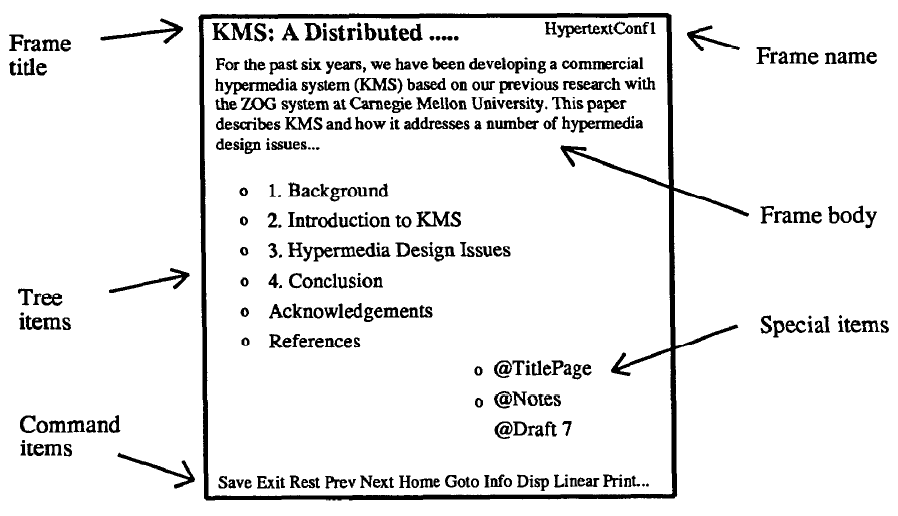
\includegraphics[scale=0.6,keepaspectratio=true]{figuras/FrameKMS.png}
    \caption{Exemplo de \textit{frame} no sitema KMS \cite{akscyn1987kms}}
    \label{fig:frameKMS}
\end{figure}

\section{Realidade Virtual}

A realidade virtual está presente quando se usa a tecnologia para criar a ilusão de que se está em um ambiente que não está lá ou não existe. Ela é uma aproximação da realidade experimentada por nós através dos nossos sentidos e sistemas de percepção. A nossa percepção da realidade vem através dos nossos sentidos. Portanto, uma vez apresentando aos sentidos às informações esperadas, sendo estas reais ou não, a nossa percepção da realidade irá se guiar por estes estímulos. Os sentidos mais comuns são visão, olfato, paladar, audição e tato. Porém também possuímos outros sentidos que afetam as nossas percepções do mundo, como por exemplo: o senso de equilíbrio, o sentimento de forças, pesos e deslocamentos sentidos por nossos membros \cite{VRS2018}.

Atualmente, a chamada realidade virtual (RV) utiliza um computador para criar um ambiente virtual tridimensional. A intenção é a de simular uma realidade apresentando os elementos desejáveis para os sentidos do usuário, visando cumprir um objetivo através da interação de um ou mais usuários com este ambiente. Estes usuários se tornam parte deste ambiente virtual, total ou parcialmente, podendo manipular objetos ou executar um conjunto de ações \cite{VRS2018}.

A RV possui uma série de usos sociais como, por exemplo, o tratamento de fobias. Há trabalhos para aracnofobia \cite{Carlin1997}, para aicmofobia ou medo de agulhas \cite{Galoustian2018}, para aerofobia ou medo de voar \cite{Rothbaum2006}, para acrofobia ou medo de altura \cite{Edwards2018} ou de forma mais geral para o medo e a ansiedade \cite{Goldman2017}. A Figura 5 ilustra a aplicação para tratamento da acrofobia. Em primeiro plano a usuária com os óculos de realidade virtual e no segundo plano o ambiente virtual simulando ambientes de escadas e plataformas com fundo transparente.

===== FIGURA ====

A indústria do entretenimento através de filmes e jogos provocou uma grande evolução de técnicas de RV que posteriormente foram aplicadas em áreas mais “sérias” como o desenvolvimento pessoal/treinamento \cite{Ma2011, Prensky2001, Smith2011}. Na prática a RV deve ser considerada como uma possibilidade sempre que o que se deseja fazer é muito perigoso, caro ou impraticável de ser realizado concretamente. Por conta destas características ela é muito usada nas áreas da educação, da saúde e militar \cite{VRS2018}. Conforme a tecnologia que permite a criação e simulação de ambientes virtuais se torna mais barata, mais aplicações são criadas com o uso destas ferramentas.

\section{Dispositivos Hápticos}

=========

\section{Modelagem de tecidos}

=========

Todos os \textit{frames} tem nomes e esse nome consiste em duas partes: uma parte alfabética e uma parte numérica. A parte alfabética é o nome do conjunto de \textit{frames} na qual pertence. O conjunto estar relacionado por um tópico específico, conforme definido pelo autor documento. Os autores têm liberdade para criar um novo conjunto de \textit{frames} sempre que criam um novo \textit{frame}. O \textit{frame} é composto de mais cinco objetos: título, corpo, itens especiais, links e itens de comando. O título (\textit{Frame title}) é utilizado nos \textit{links} quando o \textit{frame} é referenciado. O corpo (\textit{Frame body}) onde esta conteúdo textual que se deseja exibir. Os itens especiais (\textit{Special items}) são utilizados para outras informações tais com comentários, notas ou formatação das palavras. Os \textit{links} (\textit{Tree items}) são referências para outros \textit{frames}. E finalmente os itens de comandos (\textit{Command items}) são utilizados para navegabilidade entre os \textit{frames}. 

Em 1987, Campbell e Goodman apresentam o HAM \cite{campbell1987ham}, um servidor baseado em transações para um sistema de armazenamento de hipertexto. Em vez de apresentar HAM como modelo de referência, os autores apresentaram como uma máquina abstrata. O servidor é projetado para manipular vários usuários em um ambiente de rede. O sistema de armazenamento consiste em uma coleção de contextos, nós, elos e atributos que compõem um grafo de hipertexto. Desta forma, suas propriedades fornecem uma maneira de comparar recursos de diferentes sistemas de hipertexto. O modelo de armazenamento HAM aumentou abrangência do conceito de \textit{frame} do KMS com a sua maneira de armazenamento. Um grafo é o objeto HAM de nível mais alto. Ele normalmente contém todas as informações relacionadas a um tópico geral, como as informações de um projeto de software. Um gráfico contém um ou mais contextos. Os contextos podem dar suporte a configuração, histórico de versão, etc. Cada contexto tem um contexto pai e zero ou mais contextos filhos. Quando um grafo é criado, um contexto raiz inicia a árvore. O contexto que contém zero ou mais nós e elos não depende de informações contidas em seu contexto pai, resultando em uma abordagem mais organizada. Um nó contém dados do tipo texto ou códigos binários. Um elo define o relacionamento entre os nós. Enquanto o KMS agrupa informações relacionadas através de \textit{frames} com parte dos nomes iguais, o HAM possui o conceito de contexto representado por uma entidade que contém nós, links e outros contextos. 

O modelo Dexter \cite{Halasz:1994:DHR:175235.175237} origina-se do esforço para fornecer uma terminologia uniforme para representar as diferentes premissas de estruturação de hipertexto oferecidas pelos sistemas de construção de hipertexto. O núcleo do modelo é a representação ordenada de um aplicativo hipertextual em três camadas: armazenamento, parte interna do componente e de tempo de execução. A camada de armazenamento descreve a rede de nós e elos do hipertexto, sem detalhes sobre a estrutura interna e o conteúdo do nó, que é o foco da parte interna do componente. A camada de tempo de execução lida com a dinâmica e apresentação do hipertexto. Os conceitos de modelagem disponíveis na camada de armazenamento são muito básicos: os componentes descrevem informações que constituem o hipertexto e podem ser atômicas ou compostas. Links são um tipo especial de componente usado para representar caminhos navegáveis. O modelo Dexter defende muitos conceitos, como as distinções entre estrutura, navegação e apresentação de um hipertexto, cuja influência tem sido duradoura em outras áreas além do hipertexto. Assim, o modelo Dexter serve como um padrão para comparar as características e funcionalidade de vários sistemas de hipertexto (e não-hipertexto). 

Usando componentes que contêm fragmentos de texto, gráficos, imagens, animações, etc., que formam o conteúdo básico de uma rede hipertexto, o modelo Dexter também serve como uma base de princípios para desenvolver padrões de interoperabilidade e intercâmbio entre sistemas hipertexto. Várias contribuições subsequentes surgiram da crítica ao modelo Dexter e adicionaram formas mais complexas de organização de hipertexto, como por exemplo sincronização temporal entre componentes introduzida pelo modelo AHM (\emph{Amsterdam Hypermedia Model}) \cite{Hardman:1994:AHM:175235.175239} estendendo o modelo Dexter. AHM adiciona as noções de tempo, atributos de apresentação e contexto de link ao Modelo Dexter. Foi desenvolvido por Hardman, Bulterman e van Rossum (1994) para suportar o design de sistemas hipermídia que usam meios dinâmicos como áudio, vídeo e animações. Esses tipos de mídia exigem um modelo que suporte a especificação de relações temporais entre itens de dados. Desta forma, as melhorias mais importantes em relação ao Modelo Dexter são:

\begin{itemize}
 \item A especificação de apresentação de um componente atômico que inclui a especificação do canal e duração dos atributos.
 \item A especificação de apresentação inclui layout temporal, layout espacial e informações de estilo. A especificação de apresentação de um componente composto é estendida com uma lista de links de sincronização, que inclui o ID de componentes relacionados e uma relação de tempo.
 \item Componente composto não inclui conteúdo. Eles só agem como contêineres, ou seja, eles não contêm nenhum dado diretamente.
 \item Valores das âncora em componentes compostos são substituídos por uma lista de endereços indiretos (ID do componente e ID da âncora).
 \item Para cada componente filho, o AHM indica um par de ID do componente e uma hora de início.
 \item O tipo composto é especificado como paralelo ou escolha. O paralelo exibe todas as suas partes, enquanto o de escolha exibe um ou mais de seus filhos. A camada de tempo de execução implementa o mecanismo de seleção.
\end{itemize}

A Figura~\ref{fig:kindDoc} fornece uma visão de alto nível dos aspectos essenciais dos modelos hipertexto, multimídia e hipermídia. Na Figura~\ref{fig:kindDoc} (a), pode ser visto o hipertexto modelado como uma rede de componentes que são relacionados usando um conjunto de links ancorados nos componentes de origem e destino. Embora várias implementações de hipertexto possam impor restrições diferentes à estrutura interna de um componente ou à natureza exata de um conjunto de links/âncoras, todos os sistemas suportam a noção de “visitar” um componente por um período de tempo determinado pelo usuário, sendo essa visita terminada no final da aplicação ou interrompida/substituída/aumentada ao seguir um link para um ou mais componentes. Observe que o significado de visitar um componente, ou seja, exibir os efeitos visuais ao usuário, geralmente é considerado uma propriedade interna dos dados. A Figura~\ref{fig:kindDoc} (b) ilustra uma apresentação multimídia genérica. Como na Figura~\ref{fig:kindDoc} (a), a apresentação é composta por uma coleção de componentes. Ao contrário da Figura~\ref{fig:kindDoc} (a), os componentes devem ser apresentados em alguma ordem relativa definida pelo autor. A existência de tal relacionamento de ordenação depende de uma noção explícita de tempo no modelo. Enquanto o usuário ainda pode ter controle sobre a seleção de componentes a serem visitados, os componentes selecionados e apresentados podem mudar sem a intervenção direta do usuário devido a essa noção de tempo. Ou seja, o modelo não apenas define os componentes da apresentação, mas também define um relacionamento que especifica quando os componentes são apresentados um em relação ao outro. Os sistemas multimídia normalmente suportam dois tipos de recursos de navegação que fornecem ao usuário controle sobre a apresentação. O método ajusta a referência de tempo atual em uma apresentação, indicada pela linha horizontal mais forte na Figura~\ref{fig:kindDoc} (b). Usando uma interface de controle semelhante à de uma fita cassete de áudio ou de um \textit{compact disk player}, o usuário pode parar/iniciar/ avançar rapidamente/retroceder (e às vezes pesquisar) a apresentação. O segundo tipo de navegação - e menos comum - é semelhante a um link de hipertexto, indicado pela seta de ligação na Figura~\ref{fig:kindDoc} (b). Na figura, o ponto de partida desta seta pode ser chamado de âncora, que é um pedaço do conteúdo que é associado a um link. Seguir o link leva o usuário ao ponto de tempo indicado pela linha pontilhada na ilustração. Isso é essencialmente equivalente a uma operação de avanço rápido, onde, diferente deste tipo de operação, o ``ponto de partida'' e ``ponto de parada'' são definidos pelo autor do documento e não pelo usuário.

 A Figura~\ref{fig:kindDoc} (c) fornece uma descrição de alto nível de uma maneira de combinar hipertexto e multimídia: fazendo com que cada componente do modelo de hipertexto seja uma apresentação multimídia independente. Esse modelo tem dois conjuntos de interesses: aqueles relacionados à navegação hiperestruturada através do documento e aqueles relacionados à apresentação multimídia da informação. Para muitas formas simples de suporte hipermídia, o esboço da Figura~\ref{fig:kindDoc} (c) apresenta um modelo adequado de comportamento do sistema.

\begin{figure}[!ht]
    \centering
    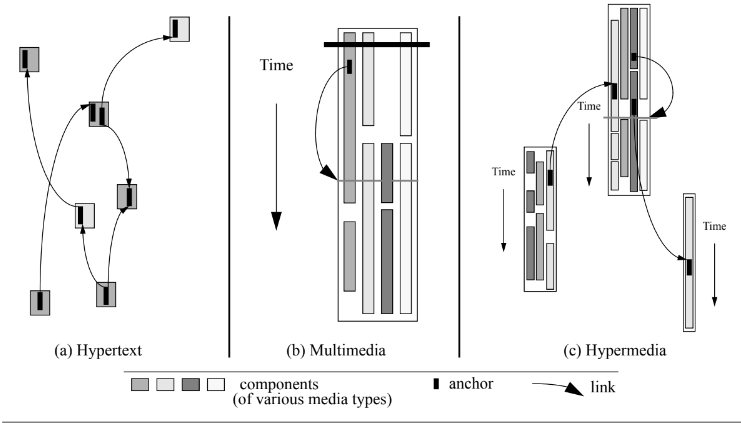
\includegraphics[scale=0.6,keepaspectratio=true]{figuras/kindsDocuments.png}
    \caption{Tipos de documentos  \cite{Hardman:1994:AHM:175235.175239}}
    \label{fig:kindDoc}
\end{figure}

Em geral, um modelo hipermídia deve ser capaz de especificar como partes individuais da informação se relacionam umas com as outras em qualquer nível que um autor de documentos ache que faria sentido. Esse nível dependeria da maneira como os dados seriam armazenados e das habilidades de apresentação/navegação dos sistemas de tempo de execução disponíveis para os usuários. A especificação de restrições de tempo dentro de um documento depende, portanto, da natureza dos elementos de dados subjacentes e da forma como estes podem ser combinados para apresentação. A estrutura interna dos dados estará além do escopo do modelo hipermídia, mas a composição dos componentes permanece central para o modelo \cite{Soares:2005qy}. A relação entre os objetos de um documento hipermídia pode ser estabelecida com o conceito de conector abordado em \cite{Muchaluat-Saade:2002aa,Muchaluat-Saade:2003aa} e que apresenta requisitos fundamentais, para especificação de documentos hipermídia. Dentre eles, estão: especificação de documentos de forma estruturada, a representação de tipos diferentes de objetos de mídia, especificação de relacionamentos espaço-temporais complexos entre componentes, a definição das características de apresentação separada da definição dos componentes, a especificação do comportamento temporal do documento de uma forma flexível e a possibilidade de adaptação do documento. Tais características são influenciadas pelo paradigma temporal adotado pelo modelo. Existem vários tipos de abordagens para a implementação temporal em um sistema hipermídia, dentre eles estão a linha do tempo e o de eventos. Na primeira abordagem, todos os objetos do documento se relacionam com a linha do tempo, ou seja, todas as ações em cima dos objeto acontecem em um determinados instantes na linha do tempo. Já na abordagem baseada a eventos, os objeto se relacionam de acordo com determinados eventos que acontecem durante a execução. Desta forma, ações iniciarão se determinado evento acontecer independente de seu instante na linha do tempo. A abordagem baseada em eventos permite que o autor defina documentos hipermídia que contenham ações associadas tanto a relações temporais e espaciais quanto a eventos assíncronos, como por exemplo interação do usuário \cite{allen1983maintaining}. O modelo NCM, detalhado na próxima seção, é baseado em eventos e por isso é usado como base para o desenvolvimento desta tese.

\section{Modelo NCM}
\label{sec:modeloNCM}

    Modelos conceituais devem ser ricos em seus recursos semânticos para representar objetos multimídia complexos e também para expressar seus requisitos de relacionamentos. Os modelos hipermídia também são o eixo das ferramentas de autoria e formatação. Esta seção é dedicada à apresentação do modelo NCM -- \textit{Nested Context Model}, fornecendo a base para a discussão sobre as facilidades de autoria e formatação realizadas nas seções a seguir. 

    O NCM, chamado de Modelo de Contextos Aninhados, possui várias entidades que representam objetos que estarão envolvidos em um documento hipermídia. Dentre elas, o modelo se baseia em nós e elos (links). Nós representam um conjunto de informação a ser apresentada enquanto que os links representam os relacionamentos entre os nós.

    Os nós são classificados em nós de composição e nós de conteúdo. Os nós de composição são nós que funcionam como repositório de outros nós, ou seja, seu conteúdo é uma lista de nós. Existe também uma especialização dos nós de composição que são os nós de contexto, estes contêm além de nós de conteúdo, uma lista de links. Estas estruturas possibilitam a organização de elementos de mídia  que se relacionam conceitualmente. Possibilitando por exemplo, definir um comportamento para todo o contexto. Para acessar um nó dentro de um nó de composição, é necessário usar a interface para um nó de composição chamada de porta. A Figura~\ref{fig:composicao} mostra uma representação de nós de contexto. As portas permitem relacionamentos de nós internos com nós externos ao contexto.
    
    \begin{figure}[!ht]
    \centering
    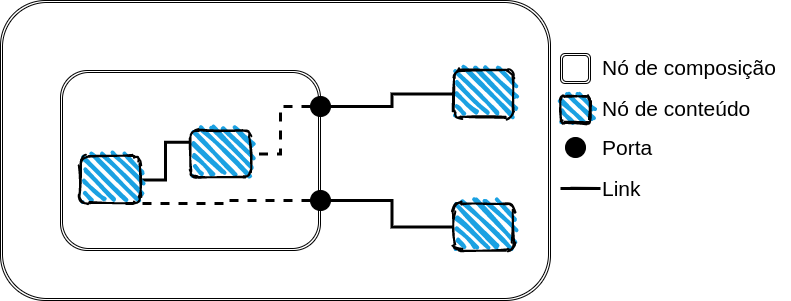
\includegraphics[scale=0.3,keepaspectratio=true]{figuras/Nocomposicao.png}
    \caption{Representação de nós de contexto \cite{Soares:2005qy}}
    \label{fig:composicao}
    \end{figure}
    
    Os nós de conteúdo possuem um conteúdo a ser apresentado para o usuário. Este conteúdo pode variar entre: texto, imagem, áudio, vídeo ou código de execução (scripts desenvolvidos em uma linguagem procedural). Um nó também pode conter variáveis de documento (conjunto de propriedades do documento). Os nós de conteúdo são acessados através de suas âncoras que podem ser de conteúdo ou de atributo. Uma âncora de conteúdo representa um subconjunto de informação do nó de conteúdo. Portanto ela pode variar de acordo com o tipo de nó ao qual ela pertence (e.g. conjunto de quadros de um vídeo, conjunto de caracteres de um texto, etc). Já a âncora de atributo representa uma propriedade do nó. A Figura~\ref{fig:NCM} mostra um visão geral simplificada do modelo NCM onde foram omitidas várias entidades e propriedades para simplificar a exposição do modelo. No decorrer deste capítulo, serão explicadas as entidades pertinentes a cada tópico.

\begin{figure}[!h]
    \centering
    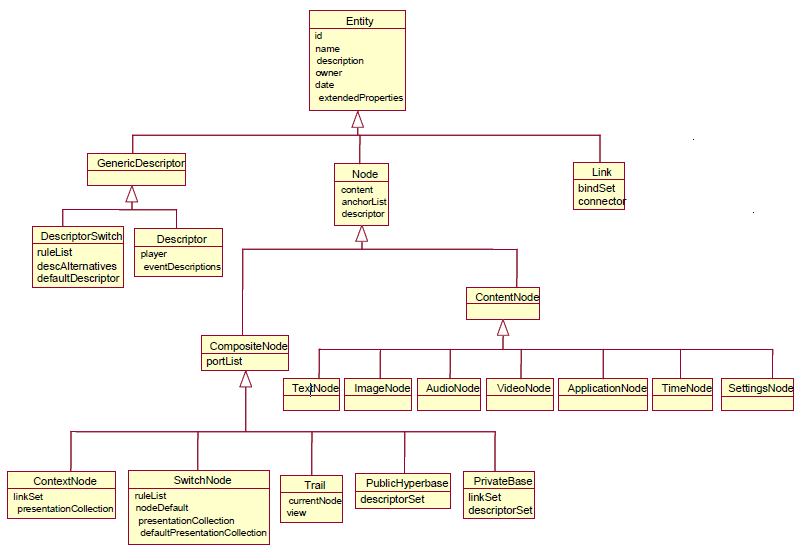
\includegraphics[scale=0.6,keepaspectratio=true]{figuras/NCM_old.png}
    \caption{Visão geral do modelo NCM \cite{Soares:2005qy}}
    \label{fig:NCM}
\end{figure}

    O link é uma entidade que materializa conexões entre nós. E essa conexão é estabelecida com duas propriedades importantes, o conector e um conjunto de associações a esse conector. O conector especifica qual tipo de relação será estabelecida. Desta forma, quando o link indicar um conector, a ligação vai seguir a especificação deste conector. Vários links podem utilizar o mesmo conector mudando os participantes da relação, havendo assim a reutilização de elementos. O NCM provê dois tipos de conectores, os causais e os de restrição. Somente os conectores causais serão abordados neste texto, eles representam uma relação de  causalidade, ou seja, quando as condições (representadas por um conjunto de papéis de condição) forem satisfeitas, um conjunto de ações deve ser executado (representado por um conjunto de papéis de ação).
    
    Modelos multimídia são geralmente comparados em termos de seu poder de expressividade, i.e., a amplitude de ideias que podem ser representadas e comunicadas nesse modelo. O arranjo temporal entre objetos de mídia em uma apresentação multimídia é  particularmente importante, portanto modelos buscam atender a um conjunto de relações temporais, que usualmente são descritas como relações temporais de Allen \cite{allen1990maintaining}. O modelo NCM pode expressar todas as relações de sincronização definidas nas relações temporais de Allen utilizando conectores. Os conectores em NCM seguem uma abordagem baseada em eventos. Desse modo, conectores permitem que NCM expresse as relações de sincronismo temporal com eventos. A Figura~\ref{fig:allen} mostra os conectores para cada relação de Allen. Adicionalmente, conectores em NCM podem representar relacionamentos assíncronos, isto é, aqueles que não se sabe quando vão acontecer. Por exemplo, relações que dependam da interação do usuário como por exemplo o conector \textit{onKeySelectionStart} que representa o evento de seleção. Assim quando o usuário selecionar (evento \textit{selection}) uma mídia do documento, pode iniciar a exibição de uma âncora (ação \textit{start}). 

\begin{figure}[!h]
    \centering
    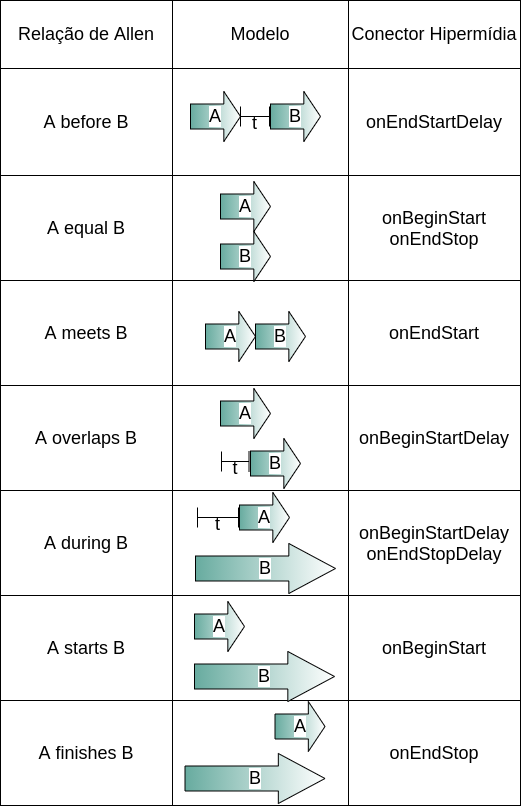
\includegraphics[scale=0.4,keepaspectratio=true]{figuras/RelacoesdeAllen.png}
    \caption{Relações de Allen \cite{allen1990maintaining} e os respectivos conectores hipermídia em NCM que as representam}
    \label{fig:allen}
\end{figure}
      

    Os links conectam os vários tipos de nós existentes no documento, representando  relações entre eles. Para que se estabeleça essa relação será necessário que o link referencie uma interface que pode ser âncora, porta ou atributo de um determinado nó. A Figura~\ref{fig:NCM_Interface} mostra os tipos de interface que o NCM contempla.

\begin{figure}[!ht]
    \centering
    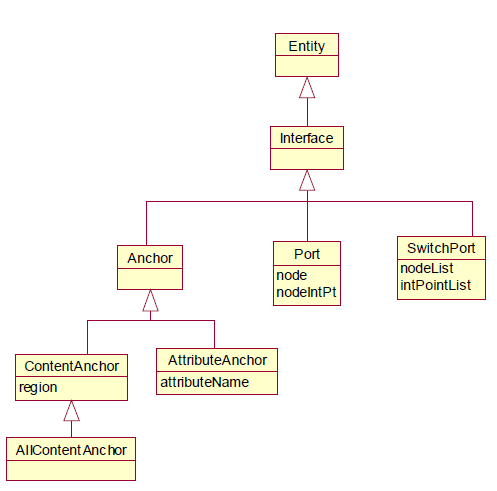
\includegraphics[scale=0.6,keepaspectratio=true]{figuras/NCM_interface.png}
    \caption{Tipos de interfaces do modelo NCM \cite{Soares:2005qy}}
    \label{fig:NCM_Interface}
\end{figure}

A Figura~\ref{fig:link}, retirada de \cite{muchaluat2003relations}, mostra um exemplo de conector e dois elos que o utilizam. O l$_1$ representa a relação entres os nós A, B e C. O conector R possui seus papeis onde pode representar condição ou ação. Na figura, se os nós A e B fazem o papel de condição, quando suas âncoras tornarem a condição satisfeita, uma ação vai acontecer na âncora do nó C.

\begin{figure}[!ht]
    \centering
    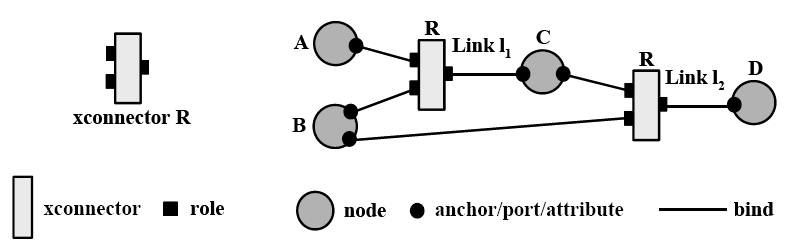
\includegraphics  [scale=0.6,keepaspectratio=true]{figuras/conector.png}
    \caption{Estrutura de Link \cite{muchaluat2003relations}}
    \label{fig:link}
\end{figure}


O modelo NCM segue o paradigma baseado em eventos. Desta forma todo o documento hipermídia é orientado a um conjunto de eventos pré definidos e extensível. Então toda condição mapeada no documento está associada a um evento. A Tabela~\ref{tab:eventosNCM} apresenta os eventos presentes no modelo NCM.

\begin{table}[!ht]
\label{tab:eventosNCM}
\caption{Eventos presentes no modelo NCM}
\centering
{
  % distancia entre a linha e o texto
  \renewcommand\arraystretch{1.25}
  \begin{tabular}{|p{5cm}|p{10cm}|} \hline
   \multicolumn{1}{|c|}{Nome} & \multicolumn{1}{c|}{Descrição}  \\ \hline 
  
    Evento de exibição & Representa a exibição de uma âncora de conteúdo (segmento de mídia) \\  \hline

    Evento de composição &  Representa a exibição da estrutura de um nó de composição \\  \hline

    Evento de seleção & Representa a seleção de uma âncora de conteúdo de um nó \\  \hline

    Evento de atribuição & Refere-se a mudança de valor de uma âncora de atributo de um nó \\  \hline

    Evento de superposição do dispositivo apontador & Representa a superposição do mouse sobre uma âncora de conteúdo de um nó \\  \hline
 
    Evento de arraste & Representa o arraste sobre uma âncora de conteúdo de um nó \\  \hline

    Evento de foco & Representa o ganho de foco de uma âncora de conteúdo de um nó \\  \hline

  \end{tabular}
}
\end{table}

À medida que os eventos vão acontecendo, eles vão mudando de estado obedecendo uma máquina de estados apresentada na Figura~\ref{fig:maqEstado}. As mudanças de estado acontecem de acordo com a execução da aplicação controlada pelo formatador \cite{rodrigues2003formataccao}. Mudanças de estado de eventos eventualmente satisfazem condições associadas aos conectores e elos, causando as respectivas ações também especificadas pelos conectores e elos.

\begin{figure}[!ht]
    \centering
    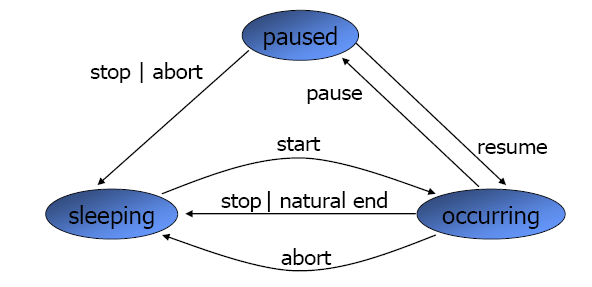
\includegraphics[scale=0.6,keepaspectratio=true]{figuras/maquinaEstadoNCM.png}
    \caption{Máquina de estados dos eventos no NCM \cite{Soares:2005qy}}
    \label{fig:maqEstado}
\end{figure}

Um evento NCM pode estar em um dos seguintes estados: dormindo (\textit{sleeping}), ocorrendo (\textit{occurring}) ou pausado (\textit{paused}). Todo evento possui um atributo denominado ocorrências (\textit{occurrences}), que armazena a quantidade de vezes que o evento muda do estado ocorrendo para o estado dormindo durante a apresentação de um documento. Os eventos de exibição e de atribuição também possuem um atributo denominado repetições (\textit{repetitions}), que apresenta a quantidade de vezes seguidas que o mesmo deve ocorrer. Acompanhando a Figura~\ref{fig:maqEstado} e tomando como exemplo um evento de exibição, o mesmo  inicia no estado dormindo. Quando há a exibição de suas unidades de informação, o evento passa para o estado ocorrendo. Caso a apresentação seja suspensa por um tempo, o evento vai para o estado pausado e permanece enquanto a situação durar. Ao final da apresentação, o evento volta para o estado dormindo, seu atributo \textit{occurrences} é incrementado de uma unidade, e o atributo \textit{repetitions} é decrementado de uma unidade, caso seja maior que zero. Se, após ser decrementado, o atributo \textit{repetitions} possuir um valor maior que zero, a apresentação do evento será reiniciada automaticamente. Quando uma apresentação de um evento é interrompida abruptamente, através de um comando de aborto da exibição, o evento passa para o estado dormindo, sem que o atributo ocorrências seja incrementado e tornando zero o valor do atributo \textit{repetitions}. Eventos de seleção permanecem no estado ocorrendo enquanto a âncora correspondente estiver sendo selecionada. De modo similar, eventos de arraste, foco e superposição permanecem no estado ocorrendo enquanto a respectiva operação sobre a âncora durar. Já os eventos de atribuição permanecem no estado ocorrendo enquanto os valores dos atributos estiverem sendo modificados. Evidentemente, eventos instantâneos, como uma simples atribuição de valor, podem permanecer por um tempo infinitesimal no estado ocorrendo.

Um evento de apresentação pode mudar do estado ocorrendo para dormindo em duas situações: quando termina a exibição da unidades de informação ou quando há uma ação que force o término do evento. A duração de um evento é o tempo que ele permanece no estado ocorrendo. No caso de um evento de apresentação, essa duração pode depender do objeto de mídia ou ser especificada pelo descritor do evento. A duração de um evento de apresentação será escolhida pelo formatador de documentos considerando detalhes do conteúdo, parâmetros do descritor, relacionamentos do documento (principalmente os elos) e outras informações externas, como características da plataforma de exibição. Um evento de apresentação associado a um nó de composição permanece no estado ocorrendo enquanto pelo menos um evento de apresentação associado a qualquer um dos nós filhos dessa composição estiver no estado ocorrendo ou enquanto pelo menos um elo filho do nó de composição estiver sendo avaliado. Um evento de apresentação associado a um nó de composição está no estado pausado se pelo menos um evento de apresentação associado a qualquer um dos nós filhos da composição estiver no estado pausado e todos os outros eventos de apresentação associados aos nós filhos da composição estiverem no estado dormindo ou pausado. Do contrário, o evento de apresentação está no estado dormindo. 

\section{Linguagem NCL}
\label{sec:LingNCL}

A Linguagem NCL (\textit{Nested Context Language}) \cite{soares2007ginga} é uma linguagem declarativa usada para especificar documentos hipermídia para TV digital interativa  compostos de objetos de mídia (e.g., Texto, imagem, gráfico, áudio, vídeo, animação) e relacionamentos entre os objetos. As linguagens declarativas têm como principal característica a semântica declarativa cujo conceito básico é a maneira simples de determinar significado de cada sentença e não depender de como será usada, ou seja, não considera os detalhes inerentes da semântica de execução. Para construção de uma linguagem de especificação de documentos hipermídia, é necessário um modelo conceitual hipermídia que expresse todas as entidades. Na literatura existem vários modelos, alguns citados no início deste capítulo, e o NCM foi utilizado pela linguagem NCL como base. Portanto, os elementos criados na linguagem NCL foram baseados nas entidades no modelo NCM. A base sintática é o XML \cite{W3C:2008aa}. A versão atual da linguagem é versão 3.0, que é suportada pelo \textit{middleware} declarativo Ginga-NCL, o formatador que executa um documento escrito em NCL. A linguagem e o formatador se tornaram padrão brasileiro de TV Digital em 2007 \cite{ABNT:2011aa} e padrão internacional para IPTV em 2009 \cite{ITU:2009ma}. Para que o autor possa construir código imperativo, poderá utilizar \textit{scripts} Lua \cite{ierusalimschy1996lua} que são referenciados por um tipo de mídia em NCL. O módulo NCLua permite que um código procedural em Lua consiga interagir com um documento hipermídia NCL \cite{sant2008nclua}.

Usando NCL, os autores podem descrever o comportamento temporal de uma apresentação multimídia, associando \textit{hyperlinks} (interação do usuário) com objetos de mídia, definindo alternativas de apresentação (adaptação) e descrevendo o layout da apresentação em múltiplos dispositivos. NCL também permite para edição de comandos do usuário, o uso de comando externos, incluindo comando para geração de aplicação em tempo de execução.

A linguagem NCL foi desenvolvida em módulos funcionais, seguindo a abordagem utilizada em várias linguagens \cite{world2006namespaces} recomendadas pelo W3C (\textit{World Wide Web Consortium}). Os módulos são conjuntos de elementos que estão reunidos a partir de conceitos relacionados e seguem listados na Tabela~\ref{tab:modulos}.

\begin{table}[!ht] \footnotesize
\caption{Módulos da Linguagem NCL 3.0 \cite{soares2009programando}}
\label{tab:modulos}
\centering
{
  % distancia entre a linha e o texto
  \renewcommand\arraystretch{0.5}
  \begin{tabular}{|p{5cm}|p{10cm}|} \hline
  \multicolumn{1}{|c|}{Módulos} & \multicolumn{1}{c|}{Identificadores} \\\hline 
 
  \textit{Animation} & http://www.ncl.org.br/NCL3.0/Animation  \\\hline
  \textit{CompositeNodeInterface} & http://www.ncl.org.br/NCL3.0/CompositeNodeInterface \\\hline
  \textit{CausalConnector} & http://www.ncl.org.br/NCL3.0/CausalConnector \\\hline
  \textit{CausalConnectorFunctionality} & http://www.ncl.org.br/NCL3.0/CausalConnectorFunctionality \\\hline
  \textit{ConnectorCausalExpression} & http://www.ncl.org.br/NCL3.0/ConnectorCausalExpression \\\hline
  \textit{ConnectorAssessmentExpression} & http://www.ncl.org.br/NCL3.0/ConnectorAssessmentExpression \\\hline
  \textit{ConnectorBase} & http://www.ncl.org.br/NCL3.0/ConnectorBase \\\hline
  \textit{ConnectorCommonPart} & http://www.ncl.org.br/NCL3.0/ConnectorCommonPart \\\hline
  \textit{ContentControl} & http://www.ncl.org.br/NCL3.0/ContentControl \\\hline
  \textit{Context} & http://www.ncl.org.br/NCL3.0/Context \\\hline
  \textit{Descriptor} & http://www.ncl.org.br/NCL3.0/Descriptor \\\hline
  \textit{DescriptorControl} & http://www.ncl.org.br/NCL3.0/DescriptorControl \\\hline
  \textit{EntityReuse} & http://www.ncl.org.br/NCL3.0/EntityReuse \\\hline
  \textit{ExtendedEntityReuse} & http://www.ncl.org.br/NCL3.0/ExtendedEntityReuse \\\hline
  \textit{Import} & http://www.ncl.org.br/NCL3.0/Import \\\hline
  \textit{Layout} & http://www.ncl.org.br/NCL3.0/Layout \\\hline
  \textit{Linking} & http://www.ncl.org.br/NCL3.0/Linking \\\hline
  \textit{Media} & http://www.ncl.org.br/NCL3.0/Media \\\hline
  \textit{MediaContentAnchor} & http://www.ncl.org.br/NCL3.0/MediaContentAnchor \\\hline
  \textit{KeyNavigation} & http://www.ncl.org.br/NCL3.0/KeyNavigation \\\hline
  \textit{PropertyAnchor} & http://www.ncl.org.br/NCL3.0/PropertyAnchor \\\hline
  \textit{Structure} & http://www.ncl.org.br/NCL3.0/Structure \\\hline
  \textit{SwitchInterface} & http://www.ncl.org.br/NCL3.0/SwitchInterface \\\hline
  \textit{TestRule}  & http://www.ncl.org.br/NCL3.0/TestRule \\\hline
  TestRuleUse & http://www.ncl.org.br/NCL3.0/TestRuleUse \\\hline
  \textit{Timing} & http://www.ncl.org.br/NCL3.0/Timing \\\hline
  \textit{TransitionBase} & http://www.ncl.org.br/NCL3.0/TransitionBase \\\hline
  \textit{Transition} & http://www.ncl.org.br/NCL3.0/Transition \\\hline
  \textit{Metainformation} & http://www.ncl.org.br/NCL3.0/MetaInformation \\\hline
 \end{tabular}
}
\end{table}

As principais entidades da linguagem NCL e que estão relacionadas com o escopo deste trabalho são: nós, elos e conectores. Cada uma delas tem um conceito a ser seguido a fim de ter a especificação de um documento com toda sua lógica de exibição. 

Como foi dito na Seção~\ref{sec:modeloNCM}, o nó na grande maioria das vezes vai conter o conteúdo a ser exibido para um usuário de aplicação multimídia. Em NCL o nó é expresso pela tag \textit{<media>} que tem entre vários atributos, o atributo src indicando o conteúdo a ser exibido. O elemento \textit{<media>} define então o que deve ser exibido. As regiões representadas pela tag \textit{<region>} definem onde será exibido o conteúdo do nó. Já os descritores informam como exibir o conteúdo do nó e são representados pela tag \textit{<descriptor>}. O momento da exibição do conteúdo é representado pelo relacionamento entre nós, que é feito por elos e conectores, com os elementos \textit{<link>} e \textit{<xconnector>} respectivamente. A Tabela~\ref{tab:areasFuncionais} mostra onde esses elementos estão distribuídos nos módulos e áreas funcionais.

\begin{table}[!ht]  \footnotesize
\caption{Algumas Áreas Funcionais da Linguagem NCL 3.0
\label{tab:areasFuncionais}
\cite{soares2009programando}}
\centering
{
  % distancia entre a linha e o texto
  \renewcommand\arraystretch{1.0}
  \begin{tabular}{|p{4.5cm}|p{6cm}|p{4cm}|} \hline
   \multicolumn{1}{|c|}{Áreas Funcionais} & \multicolumn{1}{c|}{Módulos} & \multicolumn{1}{c|}{Elementos} \\\hline 

   \multirow{3}{*}{\textit{Structure}} & \multirow{3}{*}{\textit{Structure}} & ncl\\\cline{3-3} && \textit{head}\\\cline{3-3} && \textit{body}\\\hline

   \multirow{2}{*}{\textit{Layout}} & \multirow{2}{*}{\textit{Layout}} & \textit{regionBase}\\\cline{3-3} && region\\\hline
   \multirow{2}{*}{\textit{\textit{Components}}} & \textit{Media} & \textit{media}\\\cline{2-3} & \textit{\textit{Context}} & \textit{\textit{context}}\\\hline
   
   \multirow{4}{*}{\textit{Interfaces}} & \textit{MediaContentAnchor} & \textit{area}\\\cline{2-3}
   & \textit{PropertyAnchor} & \textit{property}\\\cline{2-3}
   & \textit{CompositeNodeInterface} & \textit{port}\\\cline{2-3}
   &\multirow{2}{*}{\textit{SwitchInterface}} & \textit{switchPort}\\\cline{3-3} && \textit{mapping} \\\hline
   
   \multirow{3}{*}{\textit{Presentation Specification}} & \multirow{3}{*}{\textit{Descriptor}} & \textit{descriptor} \\\cline{3-3} 
   && \textit{descriptorParam} \\\cline{3-3} && \textit{descriptorBase} \\\hline
   
   \multirow{4}{*}{\textit{Linking}} & \multirow{4}{*}{\textit{Linking}} & \textit{bind}\\\cline{3-3} && \textit{bindParam}\\\cline{3-3} && \textit{linkParam}\\\cline {3-3} && \textit{link}\\\hline
      
   \multirow{11}{*}{\textit{Connectors}} & \multirow{10}{*}{\textit{CausalConnectorFunctionality}} & \textit{causalConnector
}\\\cline{3-3}&&
   \textit{connectorParam}\\\cline{3-3} && \textit{simpleCondition}\\\cline {3-3} && \textit{
compoundCondition}\\\cline{3-3} && \textit{
simpleAction}\\\cline{3-3} &&
   \textit{compoundAction}\\\cline{3-3} && \textit{assessmentStatement}\\\cline{3-3} &&
   \textit{attributeAssessment}\\\cline{3-3} && \textit{valueAssessment}\\\cline{3-3} &&
   \textit{compoundStatement}\\\cline{2-3} & \textit{ConnectorBase} & \textit{connectorBase} \\\hline
  
   ... & ... & ... \\\hline
   
   
  \end{tabular}
}
\end{table}

O módulo \textit{Media} define os tipos básicos de objetos de mídia. Para definir esses objetos, existe o elemento \textit{<media>}. Além do atributo id, cada objeto de mídia pode definir dois atributos principais: src, que define o URI do conteúdo e tipo do objeto. A apresentação de um documento NCL requer a sincronização de vários objetos de mídia, que são especificados por meio de elementos do tipo \textit{<media>}. Para cada objeto de mídia, um reprodutor de mídia controla a apresentação de seu conteúdo e seus eventos NCL.

Além do conteúdo a ser transmitido, o nó de conteúdo pode armazenar variáveis de ambiente como o nó de ambiente (\textit{settings node}). Esse nó representa todas as variáveis controladas diretamente pelo formatador (ferramenta responsável pela apresentação de um documento NCM). As variáveis são representadas pelos atributos (propriedades) do nó. Alguns atributos podem ter seus valores modificados por ações dos elos, outros podem ter seus valores testados inclusive pelas regras de nós \textit{switch} e de \textit{switch} de descritores, a fim de realizar a escolha entre alternativas. 

O uso do nó de ambiente é feito por meio do elemento \textit{<media>} e colocado no atributo \textit{type} a string "application/x-ncl-settings". Só pode haver apenas um em um documento NCL, cujas propriedades são variáveis globais definidas pelo autor do documento ou variáveis de ambiente reservadas (variáveis de sistema) que podem ser manipuladas pelo \textit{player} NCL. A Tabela~\ref{tab:varAmbSist} indica as variáveis de sistema já definidas, sua semântica e seus valores possíveis. Esse conjunto de variáveis é gerenciado pelo sistema receptor. Essas variáveis podem ser lidas, mas não podem ter seus valores alterados por uma aplicação NCL, um procedimento Lua ou qualquer outro procedimento imperativo ou declarativo. As aplicações nativas do receptor podem alterar os valores das variáveis e devem persistir durante o ciclo de vida do receptor.

\begin{table}[!ht] \footnotesize
\caption{Variáveis de ambiente de uma aplicação em Linguagem NCL 3.0 
\cite{soares2009programando}}
\label{tab:varAmbSist}
\centering
{
  % distancia entre a linha e o texto
  \renewcommand\arraystretch{0.5}
  \begin{tabular}{|p{4.5cm}|p{6cm}|p{4.2cm}|} \hline
  \multicolumn{1}{|c|}{Variável} & \multicolumn{1}{c|}{Significado} & \multicolumn{1}{c|}{Valores possíveis} \\\hline 

    \textit{system.language} & Idioma do áudio &  Valores definidos pela ISO 639-1 \\\hline
    \textit{system.caption} & Idioma do \textit{closed caption} &  Valores definidos pela ISO 639-1 \\\hline
    \textit{system.subtitle} & Idioma das legendas (\textit{subtitle}) & Valores definidos pela ISO 639-1 \\\hline
    \textit{system.returnBitRate}(i) & Taxa do canal interativo (i) em Kbps & real \\\hline
    \textit{system.screenSize} & Tamanho da tela do dispositivo de exibição, em linhas, pixels/linha, quando uma classe não é definida & (inteiro, inteiro) \\\hline
    \textit{system.screenGraphicSize} & Resolução configurada para o plano gráfico da tela do dispositivo de exibição, em (linhas, pixels/linha), quando uma classe não é definida & (inteiro, inteiro) \\\hline
    \textit{system.audioType} & Tipo de áudio do dispositivo de exibição, quando uma classe não é definida & “mono”|“stereo”|“5.1” \\\hline
    \textit{system.screenSize}(i) & Tamanho da tela do dispositivo (i) em (linhas,pixels/linha) & (inteiro, inteiro) \\\hline
    \textit{system.screenGraphicSize}(i) & Resolução definida para o plano gráfico do dispositivo(i) em (linhas, pixels/linha) & (inteiro, inteiro) \\\hline
    \textit{system.audioType}(i) & Tipo de áudio do dispositivo(i) & “mono”|“stereo”|“5.1” \\\hline
    \textit{system.devNumber}(i) & Número de dispositivos de exibição cadastrados na classe(i) & inteiro \\\hline
    \textit{system.classType}(i) & Tipo da classe (i) & (“passive” | “ative”) \\\hline
    \textit{system.parentDeviceRegion}(i) & Identifica o \textit{element <region>} em uma outra \textit{<regionBase>} associada ao dispositivo pai que cria o mapa de bits enviado à classe         passiva (i);nesta região, o mapa de bits também deve ser exibido & Cinco números separados por vírgulas, cada um seguindo as regras de valores associados        para   as propriedades \textit{left}, \textit{top}, \textit{width}, \textit{height}, e \textit{zIndex}, respectivamente \\\hline
    \textit{system.info}(i) & Lista de exibidores de mídia da classe (i) de dispositivos de exibição & string \\\hline
    \textit{system.classNumber} & Número de classes de dispositivos de exibição definidas & inteiro \\\hline
    \textit{system.CPU} & Desempenho da CPU em MIPS & real \\\hline
    \textit{system.memory} & Espaço de memória em Mbytes & inteiro \\\hline
    \textit{system.operatingSystem} & Tipo do sistema operacional & string \\\hline
    \textit{system.javaConfiguration} & Tipo e versão da configuração Java suportada pelo receptor JVM & string (tipo imediatamente seguido da versão, como por exemplo:         “CLDC1.1”) \\\hline
    \textit{system.javaProfile }& Tipo e versão do perfil Java suportado pelo receptor JVM & string (tipo imediatamente seguido da versão, como por exemplo: “MIDP2.0”) \\\hline
    \textit{system.luaVersion} & Versão da máquina Lua suportada pelo receptor & string \\\hline
    \textit{system.ncl.version} & Versão da linguagem NCL & string \\\hline
    \textit{system.GingaNCL.version} & Versão do ambiente Ginga-NCL & string \\\hline
    \textit{system.xxx} & Qualquer variável com o prefixo “system” deve ser reservada para uso futuro & \\\hline
 \end{tabular}
}
\end{table}

A Tabela~\ref{tab:varUser} descreve o significado e os valores possíveis das variáveis de ambiente do grupo \textit{user} no middleware Ginga-NCL, um conjunto de variáveis também gerenciado pelo sistema receptor. Assim como as variáveis da Tabela~\ref{tab:varAmbSist}, essas outras podem ser lidas, mas não podem ter seus valores alterados por uma aplicação NCL, um procedimento Lua ou qualquer outro procedimento imperativo ou declarativo. E as aplicações nativas do receptor podem alterar os valores das variáveis e devem persistir durante o ciclo de vida do receptor. A proposta de extensão desta tese, possibilita que as características do usuário seja carregadas de um arquivo profile dinamicamente, ou seja, no inicio da aplicação NCL além de poderem ser alteradas durante a execução. 

\begin{table}[!ht] \footnotesize
\caption{Variáveis de Ambiente relacionadas ao usuário de uma aplicação em Linguagem NCL 3.0 \cite{soares2009programando}}
\label{tab:varUser}
\centering
{
  % distancia entre a linha e o texto
  \renewcommand\arraystretch{0.5}
  \begin{tabular}{|p{4cm}|p{6cm}|p{5cm}|} \hline
  \multicolumn{1}{|c|}{Variável} & \multicolumn{1}{c|}{Significado} & \multicolumn{1}{c|}{Valores possíveis} \\\hline 
    \textit{user.age} & Idade do usuário & inteiro \\\hline
    \textit{user.location} & Localização do usuário (código de endereçamento postal) & string \\\hline
    \textit{user.genre} & Sexo do usuário & “m” | “f” \\\hline
    \textit{user.xxx} & Qualquer variável com o prefixo “\textit{user}” deve ser reservada para uso futuro & \\\hline
 \end{tabular}
}
\end{table}

Além dos grupos de variáveis citados na Tabela~\ref{tab:varAmbSist} e na Tabela~\ref{tab:varUser}, existem mais 6 grupos de varáveis de ambiente que fazem parte da linguagem porém não serão detalhadas neste texto por não fazerem parte do escopo deste trabalho.

A definição do relacionamento entre as mídias é feito por meio do elemento \textit{<xconnector>} representando os conectores do NCM e do \textit{<link>} representando os elos. Os relacionamentos são materializados com os links e esses referenciam conectores já estabelecidos. Um conector especifica uma relação independentemente dos objetos participantes, ou seja, ele não especifica quais nós (representados por elementos \textit{<media>, <context>, <body> e <switch>}) irão interagir através da relação. Um elemento \textit{<link>}, por sua vez, representa uma relação, do tipo definido por seu conector, interligando diferentes nós. Links que representam o mesmo tipo de relação, mas interconectam nós diferentes, podem reutilizar o mesmo conector, reutilizando todas as especificações anteriores. Um conector especifica, por meio de seus elementos filhos, um conjunto de pontos de interface, chamados papéis. Um elemento \textit{<link>} refere-se a um conector e define um conjunto de elementos \textit{<bind>}, que associam cada ponto de extremidade do \textit{link} (interface de nó) a um papel (\textit{role}) do \textit{conector} usado conforme pode-se ver na Figura~\ref{fig:linkNCL}, retirada de \cite{soares2009programando}.

\begin{figure}[!ht]
    \centering
    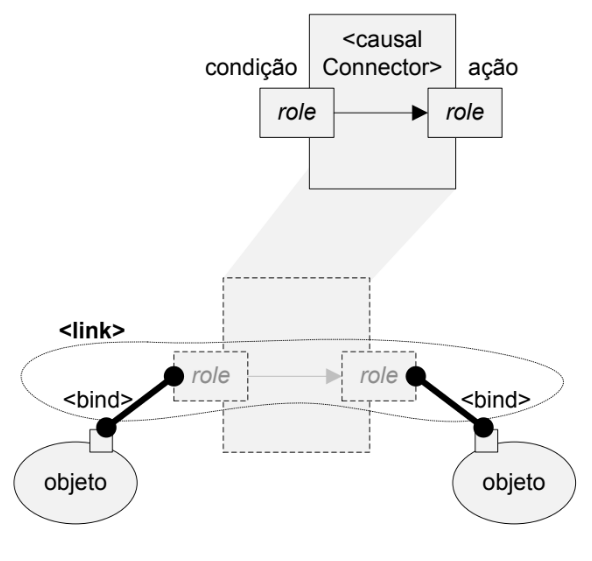
\includegraphics  [scale=0.4,keepaspectratio=true]{figuras/link.png}
    \caption{Representação do link NCL \cite{soares2009programando}}
    \label{fig:linkNCL}    
\end{figure}

Para definirmos um conector causal é necessário especificar dois papeis (\textit{roles}), um que representa a condição e outro que representa a ação ambos sobre eventos NCL. Quando a condição for satisfeita, a ação será disparada. Os links relacionam os objetos de mídia aos papeis de um conector por meio de \textit{binds}. Desta forma se um objeto de mídia estiver associado ao papel que representa a condição, isso significa que o elo vai ser disparado se o evento ocorrido estiver relacionado ao objeto ligado. De maneira análoga a ação vai acontecer sobre o objeto de mídia que estiver ligado ao papel que representa a ação.

A lista de eventos a serem monitorados por um reprodutor de mídia também deve ser computada pelo formatador NCL, levando em consideração a especificação do documento NCL. Deve obrigatoriamente verificar todos os links onde o objeto de mídia e o descritor resultante (se existir) participam. Ao computar os eventos a serem monitorados, o exibidor NCL deve obrigatoriamente levar em consideração a perspectiva do objeto de mídia, ou seja, o caminho dos elementos <\textit{body}> e dos elementos <\textit{context}> descendentes até chegar ao elemento <\textit{media}>. Apenas os links contidos nesses elementos <\textit{body}> e <\textit{context}> devem ser considerados para calcular os eventos monitorados.

Podemos ver que as relações em NCL são baseadas em eventos. Um evento é uma ocorrência no tempo que pode ser instantânea ou ter uma duração mensurável. NCL define os seguintes tipos de eventos \cite{abnt-sbtvd}:

\begin{description}
  
   \item[Apresentação] definido pela apresentação de um subconjunto das unidades de informação de um objeto de mídia, especificado em NCL pelo elemento <\textit{area}>, ou pelo próprio nó de mídia (apresentação de todo o conteúdo). Os eventos de apresentação também podem ser definidos em nós de composição (representados por um elemento <\textit{body}>, <context> ou <switch>), representando a apresentação das unidades de informação de qualquer nó dentro de um nó de composição;

   \item[Seleção] definido pela seleção de um subconjunto de unidades de informação de um objeto de mídia (que é especificado em NCL pelo elemento <\textit{area}>, ou pela âncora de conteúdo inteiro do nó de mídia), sendo apresentado e visível;
   
    \item[Atribuição] definido pela atribuição de um valor a uma propriedade de um nó (representado por um elemento <\textit{media}>, <\textit{body}>, <\textit{context}> ou <\textit{switch}>). A propriedade deve obrigatoriamente ser declarada em um elemento filho <\textit{property}> do nó.
    
    \item[Preparação] definido pelo tempo até que o conteúdo necessário para apresentação esteja disponível para o \textit{player} de um elemento <\textit{media}>.
    
   
\end{description}

O módulo \textit{CausalConnectorFunctionality} permite apenas a definição de relações causais, definidas pelo elemento <\textit{causalConnector}> do módulo \textit{CausalConnector}. Um elemento <\textit{causalConnector}> une expressões, que definem uma condição e uma ação. Quando a expressão de condição for satisfeita, a expressão de ação deve ser executada. Um conector causal  possui o atributo id, que identifica exclusivamente o elemento dentro de um documento.
Uma expressão de condição pode ser simples (elemento <\textit{simpleCondition}>) ou composta (elemento <\textit{compoundCondition}>). Ambos os elementos são definidos pelo módulo \textit{ConnectorCausalExpression}.
 
 O elemento <\textit{simpleCondition}> tem um atributo \textit{role}, cujo valor deve obrigatoriamente ser único no conjunto de \textit{roles} do conector. O \textit{role} é um ponto de interface do conector, que será associado às interfaces do nó por um link que se refere ao conector. Uma <\textit{simpleCondition}> também define um tipo de evento (atributo \textit{eventType}) e a qual transição ele se refere (atributo de transição). Os atributos \textit{eventType} e transição são opcionais. Eles podem ser inferidos pelo valor do \textit{role}, se valores reservados forem usados. Caso contrário, o \textit{eventType} e os atributos de transição precisam ser especificados.

Os valores reservados usados para definir os \textit{roles} de <\textit{simpleCondition}> são indicados na Tabela~\ref{tab:papeis}. Se um valor de \textit{eventType} for "\textit{selection}", o \textit{role} também pode definir a qual aparelho de seleção (por exemplo, teclado ou teclas de controle remoto) ela se refere, por meio de seu atributo "\textit{key}". Pelo menos os seguintes valores (diferenciando maiúsculas de minúsculas) devem ser aceitos para o atributo-chave: "0", "1", "2", "3", "4", "5", "6", "7", "8", "9", "A", "B", "C", "D", "E", "F", "G", "H", "I", "J", "K", "L", "M", "N", "O", "P", "Q", "R", "S", "T", "U", "V", "W", "X", "Y", "Z","*", "\#", "\textit{MENU}", "\textit{INFO}", "\textit{GUIDE}", "\textit{CURSOR\_DOWN}", "\textit{CURSOR\_LEFT}", "\textit{CURSOR\_RIGHT}", "\textit{CURSOR\_UP}", "\textit{CHANNEL\_DOWN}", "\textit{CHANNEL\_UP}","\textit{VOLUME\_DOWN}", 
"\textit{VOLUME\_UP}", "\textit{ENTER}", "\textit{RED}", "\textit{GREEN}", "\textit{YELLOW}", "\textit{BLUE}", "\textit{BACK}", "\textit{EXIT}", "\textit{POWER}", "\textit{REWIND}", "\textit{STOP}", "\textit{EJECT}", "\textit{PLAY}", "\textit{RECORD}", "\textit{PAUSE}". 

\begin{table}[!ht] \footnotesize
\caption{Valores de função de condição reservada associados a máquinas de estado de evento \cite{ITU:2009ma}}
\label{tab:papeis}
\centering
{
 % distancia entre a linha e o texto
 \renewcommand\arraystretch{1.0}
 \begin{tabular}{|p{4.5cm}|p{6cm}|p{4cm}|} \hline
  \multicolumn{1}{|c|}{\textit{Role Value}} & \multicolumn{1}{c|}{\textit{Transition Value}} & \multicolumn{1}{c|}{ \textit{Event Type}} \\\hline 
    \textit{onBegin} & \textit{starts} & \textit{presentation} \\\hline
    \textit{onEnd} & \textit{stops} & \textit{presentation} \\\hline
    \textit{onAbort} & \textit{aborts} & \textit{presentation}\\\hline
    \textit{onPause} & \textit{pauses} & \textit{presentation}\\\hline
    \textit{onResume} & \textit{resumes} & \textit{presentation}\\\hline
    \textit{onSelection} & \textit{starts} & \textit{selection}\\\hline
    \textit{onBeginSelection} & \textit{starts} & \textit{selection}\\\hline
    \textit{onEndSelection} & \textit{stops} & \textit{selection}\\\hline
    \textit{onBeginAttribution} & \textit{starts} & \textit{attribution}\\\hline
    \textit{onEndAttribution} & \textit{stops} & \textit{attribution}\\\hline
    \textit{onAbortAttribution} & \textit{aborts} & \textit{attribution}\\\hline
    \textit{onPauseAttribution} & \textit{pauses} & \textit{attribution}\\\hline
    \textit{onResumeAttribution} & \textit{resumes} & \textit{attribution}\\\hline
  \end{tabular}
}
\end{table}

A cardinalidade do \textit{role} especifica o número mínimo (atributo min) e máximo (atributo max) de participantes que podem desempenhar a função (número de \textit{binds}) quando o <\textit{causalConnector}> é usado para criar um <\textit{link}>. O valor mínimo de cardinalidade deve ser sempre um valor finito positivo, maior que zero e menor ou igual ao valor máximo de cardinalidade. Quando o valor de cardinalidade máxima é maior do que um, vários participantes podem desempenhar o mesmo \textit{role}, ou seja, pode haver vários \textit{binds} conectando diversos nós ao mesmo \textit{role}. O valor "\textit{unbounded}" (ilimitado) pode ser definido como o atributo max, se o \textit{role} puder ter \textit{binds} ilimitados associados a ele. Nestes dois últimos casos, um atributo qualificador deve ser especificado informando a relação lógica entre os \textit{binds} de condição simples. Conforme descrito na Tabela~\ref{tab:condSimples}, os valores possíveis para o atributo qualificador são: "ou" e "e". Se o qualificador estabelecer o operador lógico "ou", a ação do link será disparada sempre que ocorrer qualquer condição. Se o qualificador estabelecer o operador lógico "e", a ação do link será disparada depois que todas as condições simples ocorrerem.

\begin{table}[!ht] \footnotesize
\caption{Valores de qualificador de condição simples\cite{ITU:2009ma}}
\label{tab:condSimples}
\centering
{
 % distancia entre a linha e o texto
 \renewcommand\arraystretch{1.0}
 \begin{tabular}{|p{2.5cm}|p{0.8cm}|p{11cm}|} \hline
  \multicolumn{1}{|c|}{Elemento \textit{Role}} & \multicolumn{1}{c|}{Operador} & \multicolumn{1}{c|}{Significado} \\\hline 
    \textit{simpleCondition} & \textit{or} & Verdadeiro sempre que ocorrer qualquer condição simples associada. \\\hline
    \textit{simpleCondition} & \textit{and} & Verdadeiro imediatamente após todas as condições simples associadas serem verdadeiras.\\\hline
  \end{tabular}
}
\end{table}

Um atributo de atraso também pode ser definido para uma <\textit{simpleCondition}> especificando que a condição será verdadeira após um atraso de tempo a partir do momento em que ocorre a transição. O elemento <\textit{compoundCondition}> tem um atributo de operador booleano ("\textit{and}" ou "\textit{or}") relacionando seus elementos filhos: <\textit{simpleCondition}>, <\textit{compoundCondition}>, <\textit{assessmentStatement}> e <\textit{compoundStatement}>. Um atributo de atraso também pode ser definido especificando que a condição composta será verdadeira após um atraso de tempo a partir do momento em que a expressão que relaciona seus elementos filhos for verdadeira. Os elementos <\textit{assessmentStatement}> e <\textit{compoundStatement}> são definidos pelo módulo \textit{ConnectorAssessmentExpression}.

O módulo \textit{ConnectorAssessmentExpression} define quatro elementos: <\textit{assessmentStatement}>, <\textit{attributeAssessment}>, <\textit{valueAssessment}> e <\textit{compoundStatement}>.
O <\textit{attributeAssessment}> tem um atributo \textit{role}, que deve ser exclusivo no conjunto de funções do conector. Como de costume, o \textit{role} é um ponto de interface do conector, que está associado às interfaces do nó por um <\textit{link}> que se refere ao conector. Um <\textit{attributeAssessment}> também define um tipo de evento (atributo \textit{eventType}). Se o valor de \textit{eventType} for "\textit{selection}", o <\textit{attributeAssessment}> também deve definir a qual mecanismo de seleção (por exemplo, teclado ou teclas de controle remoto) ele se refere, por meio de seu atributo \textit{key}. Se o \textit{key} não for especificado, a seleção por meio de um dispositivo apontador (mouse, tela de toque, etc.) deve ser assumido. Se o valor do \textit{eventType} for "\textit{presentation}" ou "\textit{selection}", o \textit{attributeType} é opcional e, se presente, deve obrigatoriamente especificar o estado do evento ("\textit{state}"); se o \textit{eventType} for "\textit{attribution}", o \textit{attributeType} será opcional e pode ter o valor "\textit{nodeProperty}" (padrão) ou "\textit{state}". No primeiro caso, o evento representa uma propriedade do nó a ser avaliada; no segundo caso, o evento representa a avaliação do estado do evento de atribuição correspondente. Um valor de deslocamento pode ser adicionado a um <\textit{attributeAssessment}> antes da comparação. Por exemplo, um deslocamento pode ser adicionado a uma avaliação de atributo para especificar: "a posição vertical da tela mais 50 pixels". O elemento <\textit{valueAssessment}> tem um atributo de valor que pode assumir um valor de estado de evento ou qualquer valor a ser comparado com uma propriedade de nó. O elemento <\textit{assessmentStatement}> tem um atributo comparador que compara os valores inferidos de seus elementos filhos (elemento <\textit{attributeAssessment}> e elemento <\textit{valueAssessment}>). O atributo comparador deve ter um dos seguintes valores: "\textit{eq}", "\textit{ne}", "\textit{gt}", "\textit{lt}", "\textit{gte}" ou "\textit{lte}". O elemento <\textit{compoundStatement}> tem um atributo de operador booleano ("\textit{and}" ou "\textit{or}") relacionando seus elementos filhos: <\textit{assessmentStatement}> ou <\textit{compoundStatement}>. O atributo \textit{\textit{isNegated}} também pode ser definido para especificar que o elemento filho <\textit{compoundStatement}> deve ser negado antes que a operação booleana seja avaliada. Uma expressão de ação captura ações que podem ser executadas em relações causais e podem ser compostas por um elemento <\textit{simpleAction}> ou <\textit{compoundAction}>, também definido pelo módulo \textit{ConnectorCausalExpression}. O elemento <\textit{simpleAction}> tem um atributo \textit{role}, que deve ser único no conjunto \textit{roles} do conector. Como de costume, o \textit{role} é um ponto de interface do conector, que está associado às interfaces do nó por um <link> que se refere ao conector. Uma <\textit{simpleAction}> também define um tipo de evento (atributo \textit{eventType}) e qual transição de estado de evento ele aciona (\textit{actionType}). Os atributos \textit{eventType} e \textit{actionType} são opcionais. Eles podem ser inferidos pelo valor do \textit{role} se valores reservados forem usados; caso contrário, \textit{eventType} e \textit{actionType} são obrigatórios. Os valores reservados usados para definir as funções <\textit{simpleAction}> são indicados na Tabela~\ref{tab:acoes}.

\begin{table}[!ht] \footnotesize
\caption{Valores de função de ação reservados associados a máquinas de estado de evento\cite{ITU:2009ma}}
\label{tab:acoes}
\centering
{
 % distancia entre a linha e o texto
 \renewcommand\arraystretch{1.0}
 \begin{tabular}{|p{3.0cm}|p{0.8cm}|p{3cm}|} \hline
  \multicolumn{1}{|c|}{valor do Role} & \multicolumn{1}{c|}{Tipo da Ação} & \multicolumn{1}{c|}{Tipo do Evento} \\\hline 
    \textit{start} & \textit{start} & \textit{presentation}\\\hline
    \textit{stop} & \textit{stop} & \textit{presentation}\\\hline
    \textit{abort} & \textit{abort} & \textit{presentation}\\\hline
    \textit{pause} & \textit{pause} & \textit{presentation}\\\hline
    \textit{resume} & \textit{resume} & \textit{presentation}\\\hline
    \textit{set} & \textit{start} & \textit{attribution}\\\hline
    \textit{startAttribution} & \textit{start} & \textit{attribution}\\\hline
    \textit{stopAttribution} & \textit{stop} & \textit{attribution}\\\hline
    \textit{abortAttribution} & \textit{abort} & \textit{attribution}\\\hline
    \textit{pauseAttribution} & \textit{pause} & \textit{attribution}\\\hline
    \textit{resumeAttribution} & \textit{resume} & \textit{attribution}\\\hline
  \end{tabular}
}
\end{table}

Como acontece com os elementos <\textit{simpleCondition}>, a cardinalidade do \textit{role} especifica o número mínimo (atributo mínimo) e máximo (atributo máximo) de participantes que podem desempenhar o papel (número de ligações) quando <\textit{causalConnector}> é usado para criar um link. Quando o valor de cardinalidade máxima é maior que um, vários participantes podem desempenhar o mesmo \textit{role}. Quando tem o valor "\textit{unbounded}", o número de \textit{binds} é ilimitado. Nestes dois últimos casos, as ações devem ser executadas na mesma ordem de definição dos \textit{binds}.

O elemento <\textit{compoundAction}> agrupa elementos filho: <\textit{simpleAction}> e <\textit{compoundAction}>.  A execução das ações deve ser realizada na ordem em que são especificadas. Um atributo de atraso também pode ser definido, especificando que a ação composta acionada deve ser aplicada após o retardo.

O elemento <\textit{causalConnector}> pode ter elementos filhos <\textit{connectorParam}>, que são usados para parametrizar os valores de atributo do conector. O módulo \textit{ConnectorCommonPart} define o tipo do elemento <\textit{connectorParam}>, que possui atributos de nome e tipo. Para especificar quais atributos recebem valores de parâmetro definidos pelo conector, seus valores são especificados como o nome do parâmetro precedido pelo símbolo \$. Por exemplo, para parametrizar o atributo de atraso, um parâmetro chamado \textit{actionDelay} é definido (<\textit{connectorParam} \textit{name} = "\textit{actionDelay}" \textit{type} = "\textit{unsignedLong}" />) e o valor \textit{"\$actionDelay" }é usado no atributo (\textit{delay} = \textit{"\$ actionDelay"}). Os elementos do módulo \textit{CausalConnectorFunctionality}, seus atributos e seus elementos filhos devem estar de acordo com a Tabela~\ref{tab:extCausal}.

\begin{table}[!ht] \footnotesize
\caption{Módulo \textit{CausalConnectorFunctionality} estendido \cite{ITU:2009ma}}
\label{tab:extCausal}
\centering
{
 % distancia entre a linha e o texto
 \renewcommand\arraystretch{1.0}
 \begin{tabular}{|p{4cm}|p{5cm}|p{6cm}|} \hline
  \multicolumn{1}{|c|}{Elementos} & \multicolumn{1}{c|}{Atributos} & \multicolumn{1}{c|}{Conteúdo} \\\hline 
  \multirow{3}{*}{\textit{causalConnector}} & \multirow{3}{*}{id} & (\textit{connectorParam}*, (\textit{simpleCondition} |\\
                                        && \textit{compoundCondition}), (\textit{simpleAction} | \\
                                        && \textit{compoundAction}))\\\hline
   \textit{connectorParam} & \textit{name}, \textit{type} &  \textit{Empty} \\\hline

   \textit{simpleCondition} & \textit{role}, \textit{delay}, \textit{eventType},
                     \textit{key},\textit{transition}, min, max, 
                     \textit{qualifier}                  & \textit{Empty}\\\hline
                     
   \multirow{4}{*}{\textit{compoundCondition}} & \multirow{4}{*}{\textit{operator}, \textit{delay}} &       
                                        ((\textit{simpleCondition} | \\
                                        && \textit{compoundCondition})+,\\
                                        && (\textit{assessmentStatement} |\\
                                        && compo\textit{}undStatement)*)\\\hline                     
    \textit{simpleAction} & \textit{role}, \textit{delay}, \textit{eventType},
                   \textit{actionType}, \textit{value}, min, max,
                   \textit{duration}, by         & \textit{Empty}\\\hline
                   
    \textit{compoundAction} & \textit{operator}, \textit{delay} & (\textit{simpleAction} | \textit{compoundAction})+\\\hline

   \multirow{3}{*}{\textit{assessmentStatement}} & \multirow{3}{*}{\textit{comparator}} 
                                        &(\textit{attributeAssessment},\\
                                        &&(\textit{attributeAssessment} |\\
                                        && \textit{valueAssessment}))\\\hline
                                        
    \textit{attributeAssessment} & \textit{role}, \textit{eventType}, \textit{key},
                          \textit{attributeType}, \textit{offset}  & \textit{Empty}\\\hline
    \textit{valueAssessment} & \textit{value} & \textit{Empty}\\\hline
    
    \multirow{2}{*}{\textit{compoundStatement}} & \multirow{2}{*}{\textit{operator}, \textit{isNegated}}
                                & (\textit{assessmentStatement} |\\
                                && \textit{compoundStatement})+\\\hline
  \end{tabular}
}
\end{table}

O módulo \textit{ConnectorBase} define um elemento chamado <\textit{connectorBase}>, que permite agrupar conectores. O elemento <\textit{connectorBase}> deve ter o atributo id, que identifica exclusivamente o elemento em um documento. O conteúdo exato de uma base de conector é especificado pelo conjunto de conectores utilizados no documento. Porém, como a definição de conectores não é facilmente feita por usuários inexperientes, a ideia é ter usuários experientes definindo conectores, armazenando-os em bibliotecas (bases de conectores) que podem ser importadas e disponibilizando-os a terceiros para criação de links.

O elemento do módulo \textit{ConnectorBase}, representado pelo elemento <\textit{connectorBase}>, tem como atributo o \textit{id} e seus elementos filhos podem ser <\textit{importBase}> ou <\textit{causalConnector}>, com uma ou várias ocorrências desses.

\section{Exemplo de Aplicação NCL} 

A Listagem~\ref{lst:exemplo_NCL} apresenta um exemplo de uma aplicação NCL onde será exibido um vídeo de turismo
e quando chegar a um determinado momento do vídeo será exibida uma imagem de anúncio. A aplicação possui dois elementos do tipo \textit{media} um para referenciar o conteúdo do vídeo, linha 29, e outro o conteúdo de imagem, linha 33, com o anúncio de uma agência de turismo. Para especificar as características de apresentação de cada um dos nós \textit{media}, foram criadas duas regiões e os dois descritores nas linhas 5, 6, 10 e 11. 

Os relacionamentos entre os nós são representados pelo links das linhas 35 e 40. O primeiro link representa a relação que promove a exibição da imagem do anúncio em um determinado momento do vídeo. Para isso foi criado um conector causal \textit{onBeginStart} (linha 15), ou seja, quando o nó que faz o papel de \textit{onBegin} iniciar, o elemento que faz o papel de \textit{start} começará. Assim, o link da linha 35 do tipo \textit{onBeginStart} define que quando iniciar o elemento, que neste caso é uma âncora do vídeo (ancora1, definida na linha 30), o nó de imagem (imgAgencia) começará ser exibido. O link da linha 40 estabelece uma relação de término, ou seja, quando terminar o vídeo, a imagem também deixará de ser exibida.

\begin{lstlisting}[label=lst:exemplo_NCL, caption={Exemplo de uma aplicação NCL}, language=ncl]
<?xml version="1.0" encoding="ISO-8859-1"?>
<ncl id="appNcl" xmlns="http://www.ncl.org.br/NCL3.0/EDTVProfile">
<head>
    <regionBase>
        <region id="rgVideo" width="100%" height="70%" top="10%"/>
        <region id="rgPropaganda" width="40%" height="30%" top="0%"/>
	</regionBase>
	<descriptorBase>
		<descriptor id="dsVideo" region="rgVideo" explicitDur="100s"/>
		<descriptor id="dsPropaganda" region="rgPropaganda"/>
	</descriptorBase>
	<connectorBase>
		<causalConnector id="onBeginStart">
			<simpleCondition role="onBegin"/>
			<simpleAction role="start"/>
		</causalConnector>
		<causalConnector id="onEndStop">
			<simpleCondition role="onEnd"/>
			<simpleAction role="stop"/>
		</causalConnector>
	</connectorBase>
</head>
<body>
	<port id="pInicio" component="video"/>
	<media id="video" descriptor="dsVideo" src="Tour.mpg">
		<area id="ancora1" 	begin="70s" 	end="74s"/>
	</media>
	<media id="imgAgencia" descriptor="dsPropaganda" src="agencia.png" />
	<link xconnector="onBeginStart">
			<bind role="onBegin" component="video" interface="ancora1"/>
			<bind role="start" component="imgAgencia"/>
	</link>
	<link xconnector="onEndStop">
		<bind role="onEnd" component="video"/>
		<bind role="stop" component="imgAgencia"/>
	</link>
</body>
</ncl>
\end{lstlisting}

Este capítulo apresentou uma fundamentação teórica sobre Ambientes Hipermídia. Iniciou apresentando os primeiros modelos construídos para representar os ambientes hipermídia além da evolução histórica dessa representatividade. Logo em seguida o capítulo apresenta o modelo NCM e suas principais entidades e que estão relacionadas com a proposta de extensão desta tese. O capitulo finaliza apresentando os conceitos que envolvem a linguagem NCL e seus principais elementos. Alguns desse elementos serão alterados pela proposta de extensão. O próximo capítulo oferece uma visão das pesquisas relacionadas ao tema desta tese e compara-as com as proposições que foram colocadas ao longo deste trabalho. Essas pesquisas tratam da modelagem de documentos hipermídia assim como de linguagens utilizadas para a especificação dos documentos hipermídia e quais oferecem multimodal e multiusuário.